\documentclass[12pt , conference]{IEEEtran}
\usepackage{graphicx}
\usepackage{mathtools}
\usepackage{multirow}
\usepackage[justification=centering]{caption}
\usepackage{amsmath}
\usepackage{float}
\usepackage[table]{xcolor}
\usepackage[linesnumbered,ruled,vlined]{algorithm2e}
\usepackage{algpseudocode}
\usepackage{cite}
\usepackage{subcaption}
\captionsetup{font=small}
\graphicspath{}
\DeclareGraphicsExtensions{.jpg,.png}
\usepackage{fancyhdr,lipsum}
\usepackage{kantlipsum}
\newcommand\tab[1][0.5cm]{\hspace*{#1}}
\usepackage{hyperref}
\usepackage{textcomp}
\pagestyle{plain}
\setcounter{page}{1}
\usepackage[left=1cm, right=1cm, top=1.5cm,bottom=1cm,textwidth=0.5cm]{geometry}

\begin{document}

	
	\title{\large \textbf{Constraint Satisfaction Problem(CSP) \\ \large Comparative Performance Analysis of Arc-Consistency Algorithms\\AC-1, AC-2, AC-3, AC4} 			\vspace{-3ex}}
	\author
	{	Amit Roy, Roll: JH-40
		\\Department of Computer Science and Engineering,\\University of Dhaka,\\Email: \href{mailto:aroy7298@gmail.com}{aroy7298@gmail.com}
			\vspace{-3ex}
	}
	\maketitle
\fontsize{12pt}{12pt}\selectfont\noindent
	
		\section{Implementation Details:}
	In this assignment, our goal was to implement the arc consistency algorithms \textbf{(AC-1, AC-2, AC-3, AC-4)} to reduce the domain of the variables of \textbf{Constraint Satisfaction Problem(CSP)} by applying constraint propagation.\\
	According to the previously submitted concise problem definition we will have a set of \textbf{variables(eg. 50,100,150,200)} which will have a domain of random size in the range \textbf{1\texttildelow50} where the values of the domain will contain integers from the range \textbf{1\texttildelow1000}. The variables of the CSP are treated as the nodes of a graph.\\The graph is generated by a \textbf{random matrix} using \textbf{numpy}, a python library. The random adjacency matrix should be a \textbf{symmetric matrix} (i.e. if there is an edge between \textbf{u $\rightarrow$ v} there should be an edge between \textbf{v $\rightarrow$ u} ) without any self loop because all the constraints are binary constraints so we don't need edge between a node and itself. Since there is a \textbf{constraint} for every edge between  any two nodes in the graph so for \textbf{n} nodes I have generated a \textbf{n * n} adjacency matrix where the each entry of the matrix could be an integer between 0 to 11 where 0 denotes no edge and other nonzero entries denote the constraint between two adjacent nodes. I used the following constrains in my implementation:\\\\\textbf{Constraints:}
	\begin{equation}
	y \leq x
	\end{equation}
	\begin{equation}
	y \geq x
	\end{equation}
	\begin{equation}
	y=x
	\end{equation}
	\begin{equation}
	y \neq x
	\end{equation}
	\begin{equation}
	y\%x=0 \mbox{, y divides x}
	\end{equation}
	\begin{equation}
	gcd(x,y)=1 \mbox{ i.e. x and y are co-prime}
	\end{equation}
	\begin{equation}
	y=mx + c \mbox{, m and c are constants (m=2 and c = 1)}
	\end{equation}
	\begin{equation}
	y=ax^2 + bx + c \mbox{,a,b and c are constant (a=1,b=1,c=1)}
	\end{equation}
	
		For the constraints \textbf{1,2,5,7,8} we need to map them to different value for different pair of variables because they don't follow the commutative rule that is if \textbf{u$\leq$v} then \textbf{v$\geq$u} . For each algorithm, I have take 20 iterations and take the average to maintain the smoothness of the graph.
	
	\section{Comparative Performance Analysis}	To compare the performance of the arc consistency algorithms we used three performance metrics of the graph. 
	\begin{enumerate}
\item [(a)] \textit{\textbf{Running Time (msec) vs Number of nodes}}
\item [(b)] \textit{\textbf{Running Time (msec) vs Percentage of edges}}
\item [(c)] \textit{\textbf{Running Time (msec) vs domain size}}
	\\
	\end{enumerate}
	\subsection{Running Time (msec) vs Number of nodes}
	I have used the Alan Mackworth's \textbf{Consistency in Network Relations}\cite{DUMMY:1} as a source of the \textbf{AC1}, \textbf{AC2}, \textbf{AC3} algorithms and \cite{DUMMY:2} for implementing \textbf{AC4}. 
	While comparing the algorithms we have noticed that \ref{figure 1}  \textbf{AC3} performs better than \textbf{AC1}. These two algorithms are almost same except the fact that \textbf{AC1} checks consistency of all the arcs even if only one edge is revised. But \textbf{AC3} checks the consistency only the adjacent edges of the first node of the revised edge.So, it's a reason behind \textbf{AC3} performing better another reason is when the domain of any node is empty \textbf{AC3} terminates.\textbf{AC2} also performs better than \textbf{AC1} but it's performance is almost same \textbf{AC3} in most of the cases. While \textbf{AC3} almost always better than \textbf{AC4}\cite{DUMMY:3} because AC4 takes a lot of time while pre-processing. 
	\\
	\subsection{Running Time (msec) vs Percentage of edges}
	As I have increased the percentage of edges in the graph keeping the number of nodes fixed(eg. 100,200). I got the same result as the previous one. The running time of \textbf{AC3} and \textbf{AC1} is quite better than the \textbf{AC2} and \textbf{AC4}. For \textbf{AC1} and \textbf{AC3} we have noticed that their performance are almost similar for small percentage of edges but when edge percentages then \textbf{AC3} performs slightly better than \textbf{AC1}. But \textbf{AC2} and \textbf{AC4} are not so good even for small edge percentages.
	\\
	\subsection{Running Time (msec) vs Domain Size}
	According to the graph \ref{figure 3}, \textbf{AC4} performs worse than other algorithms in average case but performs better in the worst case. \textbf{AC4} performs worse for the large domains but \textbf{AC1},\textbf{AC2} and \textbf{AC3} performs almost similar for the large domain.
	
	
	\begin{table*}[ht]
		\large
		\centering
		\captionsetup{singlelinecheck = false, format= hang,  font=footnotesize, labelsep=space}
		\caption{\small : Descriptive statistics of k=4 independent treatments:	}
		\begin{tabular}{|l|l|l|l|l|l|}
			\hline
			Treatment    $\to$                                                                   & AC1        & AC2         & AC3        & AC4          & Pooled Total \\ \hline
			observations N                                                                  & 101        & 101         & 101        & 101          & 404          \\ \hline
			sum $\sum$ \textit{x$ _{i} $}                         & 961.4854   & 1,117.2210  & 650.8736   & 4,131.0253   & 6,860.6053   \\ \hline
			mean $\overline{x}$  & 9.5197     & 11.0616     & 6.4443     & 40.9012      & 16.9817      \\ \hline
			sum of squares $\sum$ \textit{x$ _{i} ^{2} $}               & 9,195.8574 & 12,393.0952 & 4,201.5039 & 169,963.7484 & 195,754.2049 \\ \hline
			sample variance \textit{s$^{2} $} & 0.4285     & 0.3485      & 0.0708     & 9.9969       & 196.6489     \\ \hline
			sample std. dev. \textit{s}                                                              & 0.6546     & 0.5903      & 0.2662     & 3.1618       & 14.0232      \\ \hline
			std. dev. of mean \textit{SE$ _{\overline{x}}$}               & 0.0651     & 0.0587      & 0.0265     & 0.3146       & 0.6977       \\ \hline
		\end{tabular}
		\label{figure 4}
	\end{table*}
	

	
	
	\noindent
	\begin{figure}[h]
		\centering
		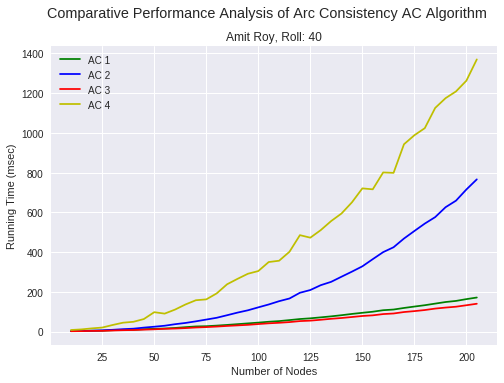
\includegraphics[width=7cm]{running_time_node_200.png}
		\captionsetup{singlelinecheck = false, format= hang,  font=footnotesize, labelsep=space}
		\caption{Running time vs number of nodes (1\texttildelow200)}
		\label{figure 1}
	\end{figure}
	
	
	\begin{figure}[h]
		\centering
		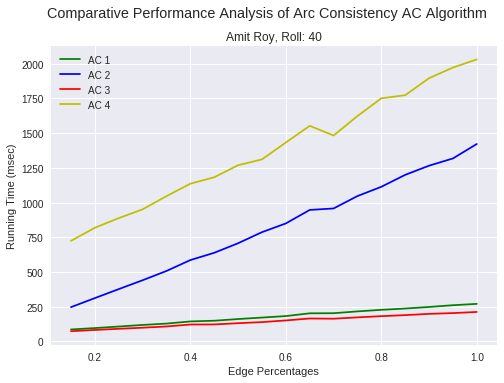
\includegraphics[width=7cm]{running_time_edge_200.png}
		\captionsetup{singlelinecheck = false, format= hang,  font=footnotesize, labelsep=space}
		\caption{Running Time vs Edge Percentage  (Nodes: 200)}
		\label{figure 2}
	\end{figure}



		\begin{figure}[h]
		\centering
		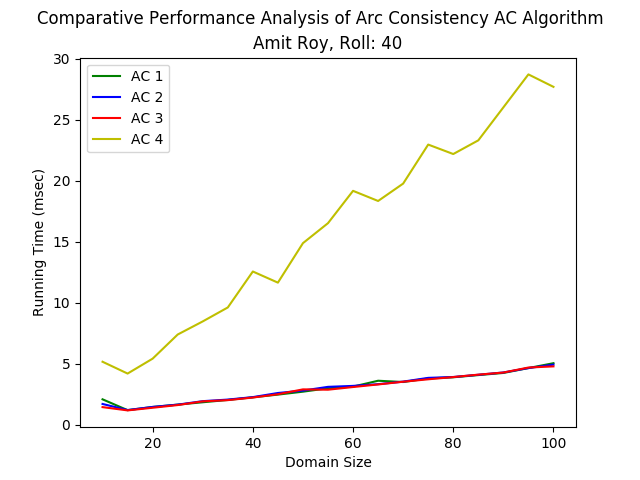
\includegraphics[width=7cm]{domain_size.png}
		\captionsetup{singlelinecheck = false, format= hang,  font=footnotesize, labelsep=space}
		\caption{Running Time vs Domain Size\\ (Nodes: 30, Edge Probability: 0.5)}
		\label{figure 3}
	\end{figure}
	

	
	\begin{table}[h]
		\fontsize{12}{11}
		\captionsetup{singlelinecheck = false, format= hang,  font=footnotesize, labelsep=space}
		\caption{\small 
			: Tukey HSD results	}
		\begin{tabular}{|l|l|l|l|l|}
			\hline
			\begin{tabular}[c]{@{}l@{}}Treatments \\ Pair\end{tabular} & \begin{tabular}[c]{@{}l@{}}Tukey HSD \\ Q statistic\end{tabular} & \begin{tabular}[c]{@{}l@{}}Tukey HSD \\ p-value\end{tabular} & \begin{tabular}[c]{@{}l@{}}Tukey HSD \\ inferfence\end{tabular} & Result      \\ \hline
			AC1 vs AC2                                                 & 9.4113                                                           & 0.0010053                                                    & ** p\textless{}0.01                                             & Significant \\ \hline
			AC1 vs AC3                                                 & 18.7706                                                          & 0.0010053                                                    & ** p\textless{}0.01                                             & Significant \\ \hline
			AC1 vs AC4                                                 & 191.5389                                                         & 0.0010053                                                    & ** p\textless{}0.01                                             & Significant \\ \hline
			AC2 vs AC3                                                 & 28.1819                                                          & 0.0010053                                                    & ** p\textless{}0.01                                             & Significant \\ \hline
			AC2 vs AC4                                                 & 182.1276                                                         & 0.0010053                                                    & ** p\textless{}0.01                                             & Significant \\ \hline
			AC3 vs AC4                                                 & 210.3095                                                         & 0.0010053                                                    & ** p\textless{}0.01                                             & Significant \\ \hline
		\end{tabular}
		\label{figure 5}
	\end{table}
	\newpage
\section{Results and Findings}	
	\noindent
	Since all the algorithms reduce the domain of the variables by eliminating inconsistent values from the domain, all algorithms will return the \textbf{same domain} if the input graph has a consistent solution. But when the input graph is not consistent then, different algorithms may return different domain due to the termination when some of the variable's domain is empty.\\To verify the correctness of the implementation, I have run all 4 algorithms for small input until finding a consistent graph. What we have noticed is all 4 algorithms provide same domain for each variable/node. which proves the correctness of the implementation. I have run all the algorithms in the platform \textbf{``google colab"}. You can find and test the implementation \href{https://tinyurl.com/solutionAC-040}{here}\\I have also performed \textbf{Anova's test with HSD tuckey} \ref{figure 4} \ref{figure 5} on my data of the running time vs number of edges for 50 nodes and edges in range (100\texttildelow200) Here, A,B,C,D corresponds to AC1,AC2,AC3,AC4. It shows significant results comparing among all the results. 
	
	
	\bibliography{bibTex} 
	\bibliographystyle{ieeetr}
	
\end{document}
